
\documentclass[a4paper]{article}
\usepackage[fontset=fandol]{ctex}
\usepackage{amsmath,amssymb}
\usepackage{graphicx}
\usepackage[margin=2.3cm]{geometry}
\usepackage[most]{tcolorbox}
\usepackage{listings}
\usepackage{hyperref}
\usepackage{booktabs}
\usepackage{float}
\usepackage{xcolor}
\lstset{language=Python,basicstyle=\ttfamily\small,keywordstyle=\color{blue},stringstyle=\color{red!60!black},commentstyle=\color{green!50!black},breaklines=true,frame=single,numbers=left,numberstyle=\tiny\color{gray}}
\newtcolorbox{knowledgebox}[1]{enhanced,colback=blue!5!white,colframe=blue!70!black,colbacktitle=blue!70!black,coltitle=white,fonttitle=\bfseries,title=#1,sharp corners}
\newtcolorbox{importantbox}[1]{enhanced,colback=yellow!10!white,colframe=yellow!70!black,colbacktitle=yellow!70!black,coltitle=black,fonttitle=\bfseries,title=#1,sharp corners}
\newtcolorbox{warningbox}[1]{enhanced,colback=red!5!white,colframe=red!70!black,colbacktitle=red!70!black,coltitle=white,fonttitle=\bfseries,title=#1,sharp corners}
\begin{document}
\begin{titlepage}
\centering
{\Large 课程讲义\par}
\vspace{1.2cm}
{\huge\bfseries Multimodal Agents: From Perception to Action\par}
\vspace{0.6cm}
{\Large CS294/194-280: Advanced Large Language Model Agents\par}
\vspace{0.4cm}
{\large Caiming Xiong, Salesforce AI Research\par}
\vspace{0.4cm}
{\large 中文教材化讲义 / Harness Build\par}
\vspace{0.8cm}
\includegraphics[width=0.84\textwidth,height=0.38\textheight,keepaspectratio]{cover.jpg}\par
\vfill
\begin{tcolorbox}[width=0.92\textwidth,colback=black!2!white,colframe=black!60,sharp corners]
\textbf{课程页}：\url{https://rdi.berkeley.edu/adv-llm-agents/sp25}\par
\textbf{录播}：\url{https://www.youtube.com/live/n__Tim8K2IY}\par
\textbf{Slides}：\url{https://rdi.berkeley.edu/adv-llm-agents/slides/Multimodal_Agent_caiming.pdf}\par
\textbf{核心 readings}：OSWorld / AGUVIS
\end{tcolorbox}
\end{titlepage}
\tableofcontents
\newpage

\section{本讲学习目标}

本讲的标题是“从感知到动作”，但真正要回答的问题是：当 agent 进入真实 computer environment 之后，感知、grounding、reasoning、action 与 memory 应该如何被系统性设计。读完后，读者应当能够：
\begin{itemize}
\item 区分 \textbf{web benchmarks}、\textbf{OS / computer-use benchmarks}、\textbf{GUI grounding benchmarks} 和 \textbf{long-video benchmarks} 的任务对象与评测哲学。
\item 解释为什么 \textbf{OSWorld} 把 task config、execution-based evaluation 和多 app workflows 放在 benchmark 的中心。
\item 说明 \textbf{AgentTrek}、\textbf{CoTA/TACO} 这类数据与训练方案分别在解决什么瓶颈。
\item 理解 \textbf{AGUVIS} 为什么要强调 pure-vision observation、统一 action space 和 inner monologue。
\item 解释 \textbf{xGen-MM-Vid} 与 \textbf{GenS} 如何把 long-video memory / grounding 连接回 multimodal agent 的设计问题。
\end{itemize}

\section{从 benchmark taxonomy 到真实 computer-use agents}

\subsection{为什么“computer use”不是普通 web automation 的别名}

讲者开篇用一组 benchmark taxonomy 做了很重要的铺垫：coding agents、web agents、mobile agents、physical agents。这个 taxonomy 不是为了罗列论文，而是为了说明 \textbf{computer tasks 往往跨越多个 app、多个界面和多个状态通道}。例如更新账本、改代码、处理文件、查网页、切换表格和浏览器，这些都不是单一网站里的 click sequence。

因此，“computer use” 比“web navigation”更广。它的 environment 包括操作系统、任意 app、文件 I/O、terminal 输出、跨窗口切换和多 app workflow。很多旧 benchmark 要么只有 demonstrations，要么只有静态状态，要么只覆盖某个子域，于是很难真正回答：\textbf{agent 是否能像人类那样在真实电脑上完成开放式任务？}

\subsection{OSWorld：真实 computer environment + execution-based evaluation}

\begin{figure}[H]
\centering
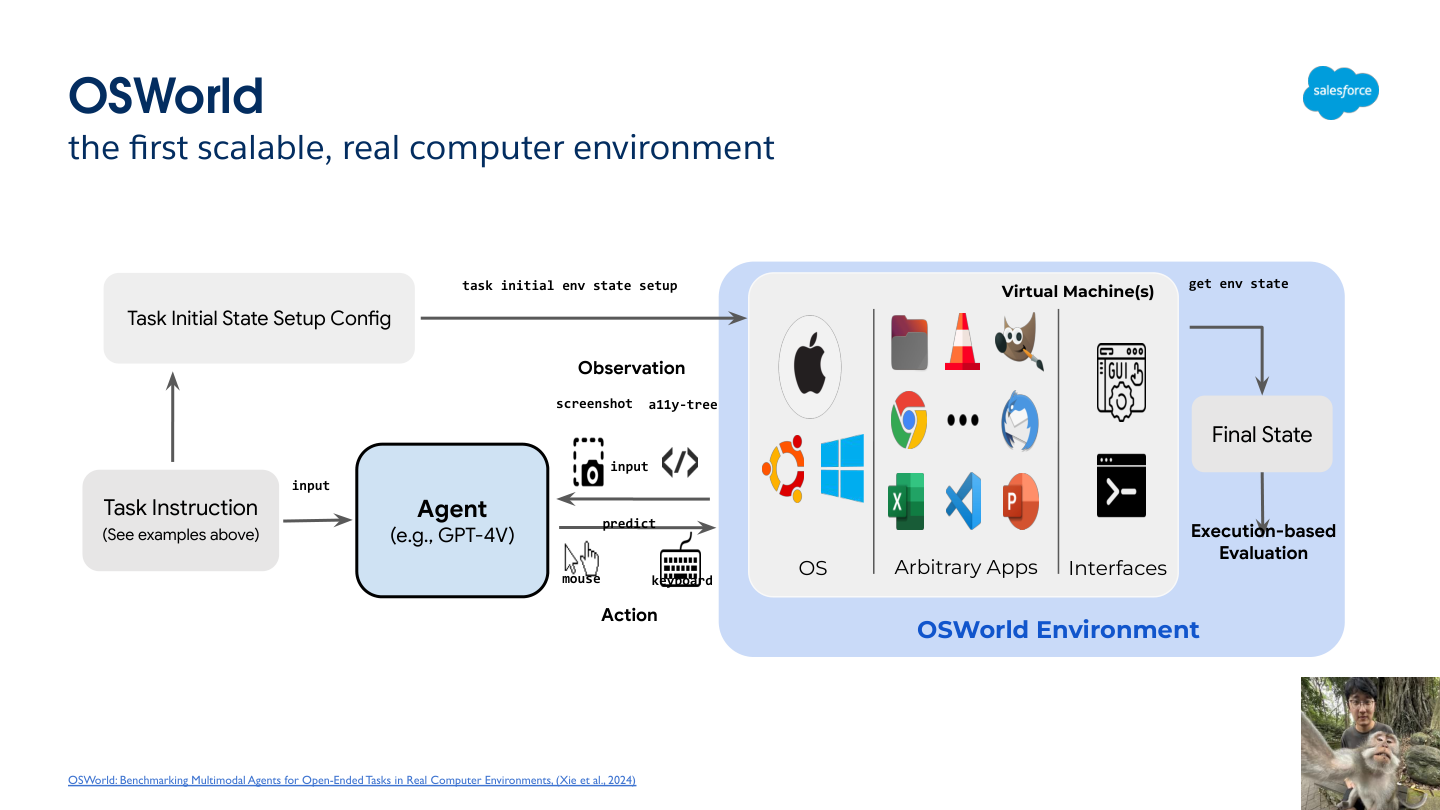
\includegraphics[width=0.84\textwidth]{figures/lec07_fig_001.png}
\caption{OSWorld 把 task instruction、virtual machine、observation 与 execution-based evaluation 放在同一个真实 computer environment 中。}
\end{figure}

OSWorld 的核心贡献，是把 environment realism 和 evaluation reliability 一起做出来。它不是只给几段轨迹，而是提供：
\begin{itemize}
\item task initial state setup config，用于还原任务开始时的虚拟机状态；
\item 统一的真实 computer environment，可容纳 arbitrary apps；
\item execution-based evaluation script，用于判断任务是否真正完成；
\item 覆盖 open domains、多 app workflows、OS file I/O 的 369 个真实任务。
\end{itemize}

这使得任务可以自然写成一条 interaction loop：
\begin{figure}[H]
\centering
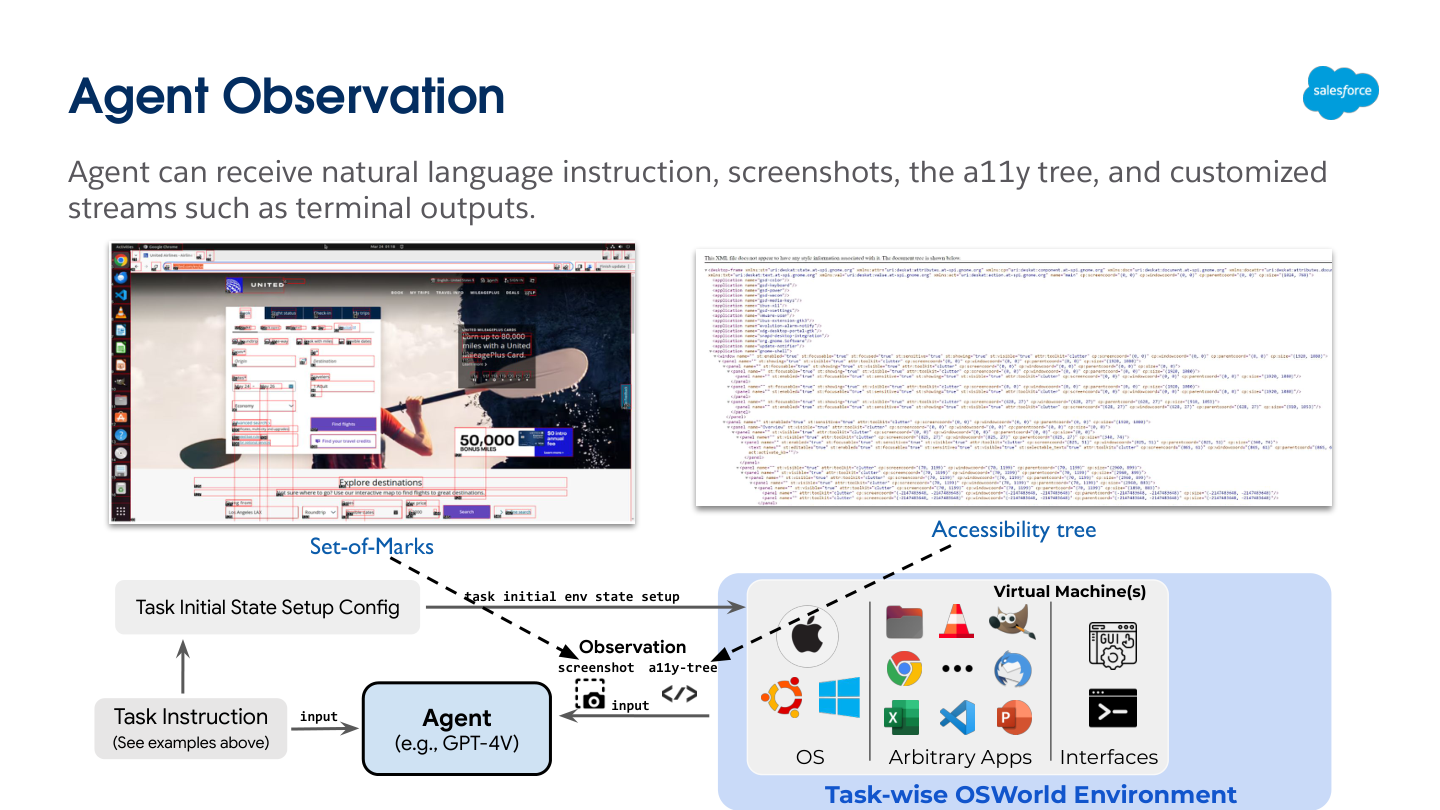
\includegraphics[width=0.80\textwidth]{figures/lec07_fig_002.png}
\caption{OSWorld 中 agent 的观测可以同时包括 screenshot、a11y tree 和其它 environment streams。}
\end{figure}

\begin{figure}[H]
\centering
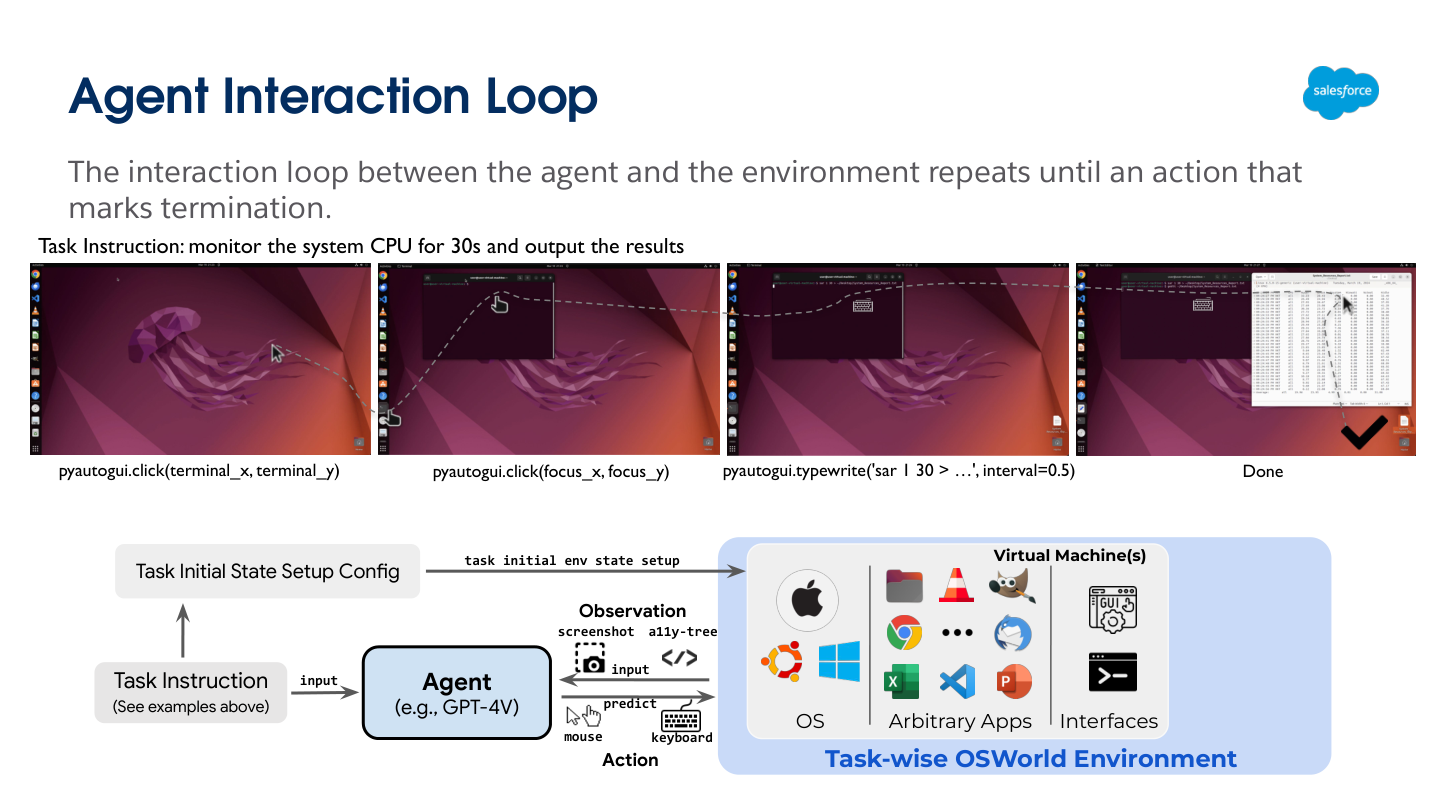
\includegraphics[width=0.80\textwidth]{figures/lec07_fig_003.png}
\caption{Instruction、observation、action、termination 和 evaluation 共同构成 OSWorld 的 interaction loop。}
\end{figure}

教材化地看，OSWorld 的最重要贡献在于：它把 reward / success 从“字符串匹配”改成了 \textbf{execution-based correctness}。可以写成
\[
R(\tau)=\mathbf{1}[\operatorname{Eval}(s_T, \tau)=\mathrm{success}],
\]
其中 $\tau$ 是整条 trajectory，$s_T$ 是最终环境状态，$\operatorname{Eval}$ 是 task-specific 的 evaluation function。这样做的意义是，它允许存在 \emph{multiple correct trajectories}，而不必假设每个任务只有一种唯一文本答案。

\begin{importantbox}{为什么这个区别很关键}
很多 computer tasks 的“答案”不是一句文本，而是某个文件是否被改对、某个应用状态是否被正确设置、某个工作流是否真的执行完。没有 execution-based evaluation，就无法严格比较 agent 与 human workflows。
\end{importantbox}

\section{OSWorld 的 baseline 结果说明了什么}

\subsection{当前 multimodal agents 仍远不是可靠的 digital assistants}

OSWorld reading 和 lecture slides 都给出同一个结论：当前最强 agent 与人类之间有非常大的差距。论文摘要里 humans 大约能完成 72.36\% 的任务，而强 baseline 约为 12.24\%。这个 gap 说明问题并不是“模型偶尔点错按钮”，而是系统级能力远未成熟。

\begin{figure}[H]
\centering
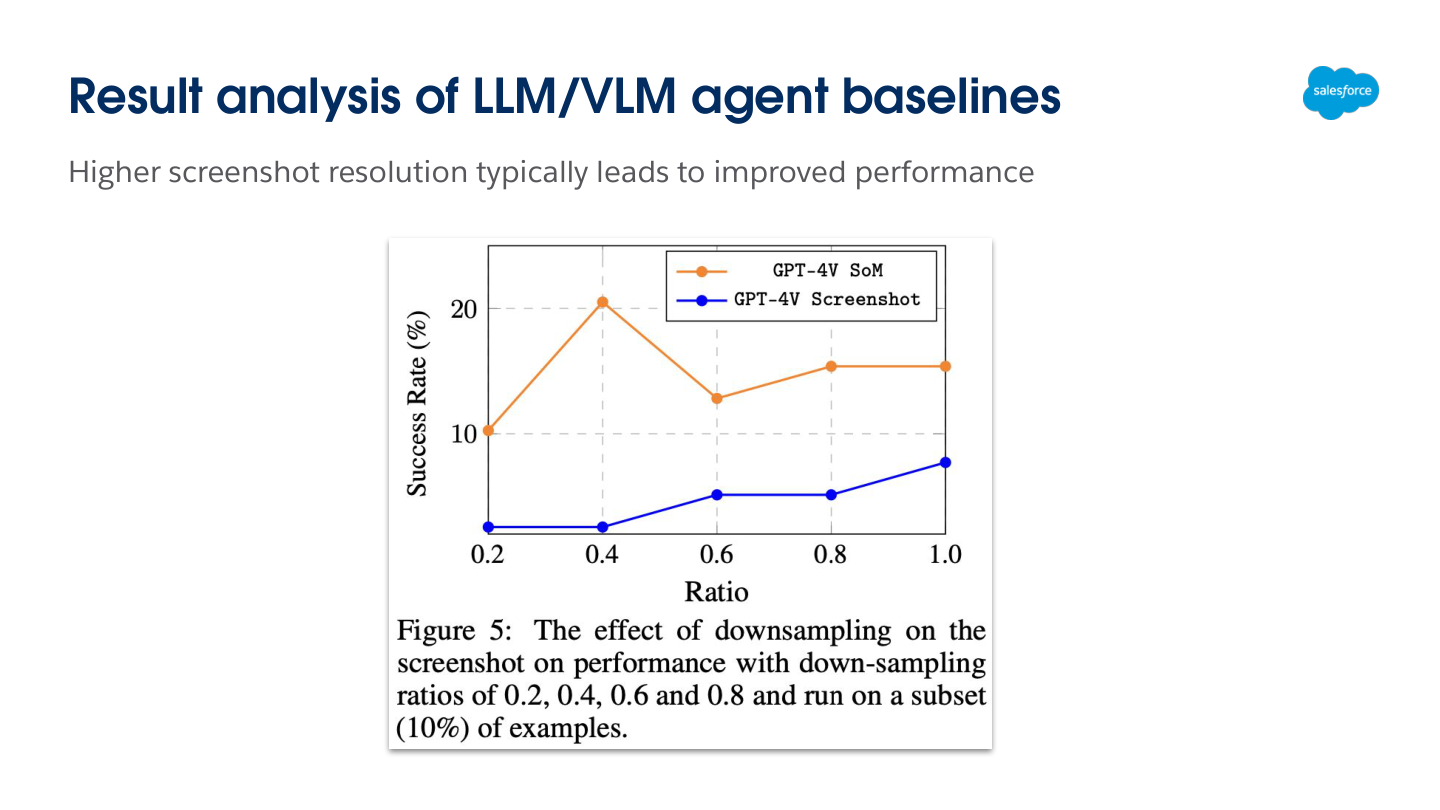
\includegraphics[width=0.76\textwidth]{figures/lec07_fig_004.png}
\caption{OSWorld baseline analysis: 分辨率、history 与 observation mode 都有影响，但距离 robust computer use 仍非常远。}
\end{figure}

slides 的分析特别值得展开成教材。它指出：
\begin{itemize}
\item 更高截图分辨率通常有帮助，因为很多 GUI 决策依赖细粒度视觉线索。
\item 更长的 text-based trajectory history 通常也有帮助，因为它改善了状态跟踪；但 screenshot-only history 的收益没那么稳定，而且会带来效率问题。
\item 模型在不同 OS 上的表现相关性很强，这说明它们遇到的是更底层的 \textbf{GUI grounding 与 operational knowledge} 问题，而不只是某个系统特有 API 的问题。
\end{itemize}

\subsection{这里的 benchmark distinction 不能被抹平}

这一段最容易被错误总结成“大家都在做 GUI agents”。这不够精确。必须区分：
\begin{itemize}
\item \textbf{Mind2Web / WebArena / VisualWebArena} 主要是 web-domain agents；它们强调网页环境、HTML 或视觉网页线索。
\item \textbf{OSWorld} 是 open-ended real computer environment；它跨 app、跨 OS，并有明确的 execution-based setup 和 evaluation。
\item \textbf{ScreenSpot} 一类数据更偏 GUI grounding benchmark，本身不等于 interactive environment。
\item \textbf{Browser Use / AndroidWorld / Mind2Web-live} 等则在 online evaluation 维度补充特定平台或部署场景。
\end{itemize}

这个 distinction 很重要，因为它直接影响模型应当优化什么能力：是网页导航、跨 app workflow、视觉 grounding，还是实时 online robustness。

\section{训练瓶颈：为什么 agent data 比语言数据更稀缺}

\subsection{AgentTrek：从教程文本到可回放轨迹}

讲者随后把重点转向训练数据。问题很直接：LLM 的成功高度依赖海量现成文本，但 computer-use agents 需要的是带环境状态与动作序列的 trajectories，这类数据没有自然规模化的网页爬取版本。于是 \textbf{AgentTrek} 的思路变得自然：既然互联网有大量 step-by-step GUI tutorials，为何不把它们转成可用的 agent training source？

\begin{figure}[H]
\centering
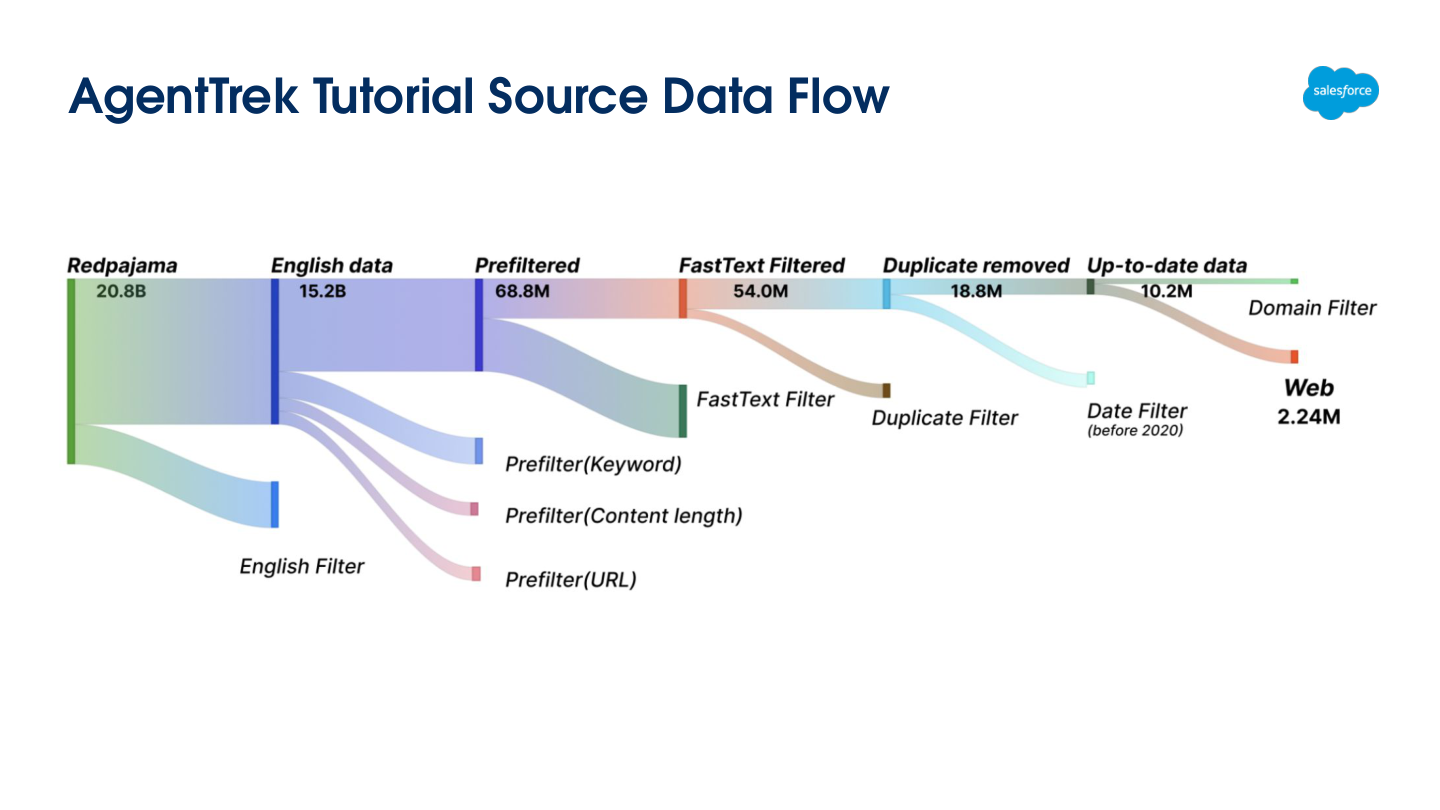
\includegraphics[width=0.80\textwidth]{figures/lec07_fig_005.png}
\caption{AgentTrek 从 web tutorials 中抽取 task structure，再用 guided replay 合成 trajectories。}
\end{figure}

它的关键不在“把教程复制给模型”，而在于 \textbf{guiding replay}：先从教程中提炼平台、环境、任务描述和关键步骤，再把这些信息转进目标环境，合成更接近真实 interaction 的轨迹。这种方法的价值在于：
\begin{itemize}
\item 教程本身已经包含了人类如何完成 GUI tasks 的结构性先验。
\item GUI tutorials 广泛存在于互联网，因此有潜在的规模优势。
\item 它能把 \emph{knowledge-rich instructions} 转成 \emph{actionable trajectories}。
\end{itemize}

但它也有边界。教程经常针对特定版本、特定布局、特定语言环境；一旦 replay 环境变化，distribution shift 就会出现。因此 AgentTrek 更像一种 \textbf{data bootstrapping mechanism}，而不是终极答案。

\section{从 CoT 到 CoTA：为什么 multimodal action model 需要 action-call capability}

\subsection{TACO / CoTA 的核心思想}

slides 接着提出一个尖锐问题：多模态 LLM 自身是否需要 \textbf{action call capability}？如果答案是肯定的，那么光靠 few-shot prompting 往往不够，因为模型需要学的不是“如何说出一个理由”，而是“如何在 reasoning 与 action 之间切换”。

\begin{figure}[H]
\centering

\includegraphics[width=0.80\textwidth]{figures/lec07_fig_006.png}
\caption{Synthetic CoTA pipeline 同时生成 thought 和 action，使模型学会 multimodal reasoning with tools/actions。}
\end{figure}

这就是 TACO / CoTA 的设计直觉。与普通 Chain-of-Thought 相比，它不是只让模型生成 $t_{1:m}$ 这类 reasoning trace，而是联合生成 $(t_{1:m}, a_{1:n})$：
\[
\max_\theta \sum_{(x, t, a)} \log p_\theta(t_{1:m}, a_{1:n} \mid x).
\]
这里 $x$ 是多模态输入与任务指令，$t_{1:m}$ 是 thought tokens，$a_{1:n}$ 是 action sequence。直觉上，CoTA 让模型学到的不是“看完图后多解释一点”，而是“什么时候该 reasoning，什么时候该 call 一个 action，动作之后如何继续 reasoning”。

\begin{lstlisting}
sample multimodal task
generate thought-and-action trace
filter useless actions
finetune multimodal action model on CoTA data
\end{lstlisting}

\subsection{质量比数量更重要}

这一段的实验结论很值得教材化，因为它提供了关于 agent training data 的一个普遍原则：\textbf{quality >> quantity}。slides 指出，小而高质量的 CoTA 数据集反而可能比混杂 Direct / CoT / CoTA 示例的大数据集更有效；把 \emph{action-useless} 数据过滤掉，也会带来收益。

这个结论说明：对 agent 来说，数据是否真的对 \textbf{action grounding 与 deployment behavior} 有帮助，比数据量本身更关键。很多普通视觉问答或纯描述性数据，并不能自然转化为更强的 computer-use behavior。

\section{AGUVIS：Unified Pure Vision Agents}

\subsection{为什么要反对异构文本 GUI 表示}

\begin{figure}[H]
\centering
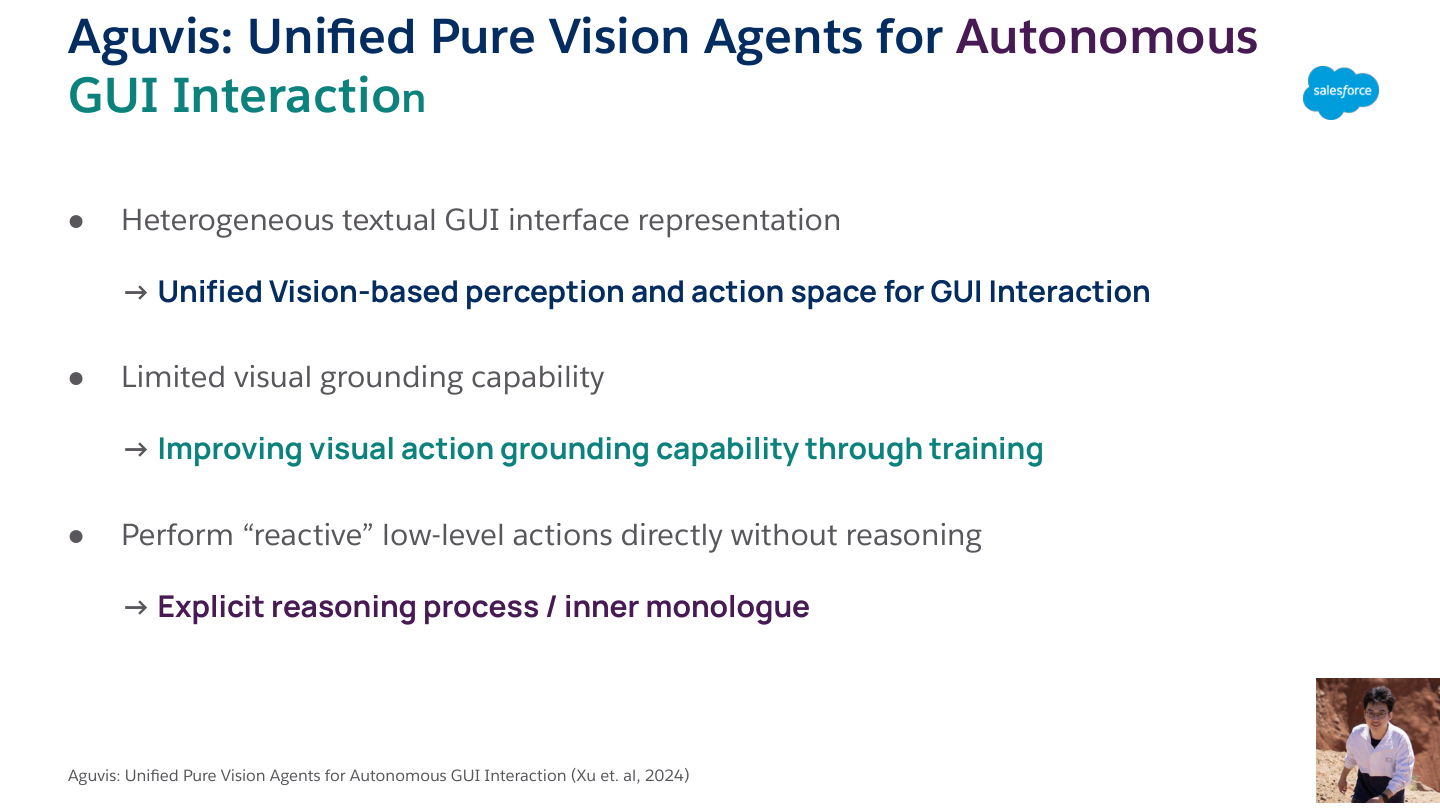
\includegraphics[width=0.80\textwidth]{figures/lec07_fig_007.png}
\caption{AGUVIS 的立场是：直接在图像 observation 上做 GUI interaction，而不是依赖 HTML / AXTree / XML 等异构文本表示。}
\end{figure}

讲者介绍 AGUVIS 的时候，重点不是模型规模，而是 problem formulation。它指出当前 GUI agents 常见的四个障碍：
\begin{itemize}
\item 依赖 HTML、AXTree、XML 等平台特有文本表示，导致 observation 不统一。
\item action space 在 web、desktop、mobile 上异构，难以做跨平台学习。
\item visual grounding 能力不足，导致模型知道该做什么却点不到正确目标。
\item 很多方法只做 \textbf{reactive low-level actions}，缺乏显式 reasoning 与 planning。
\end{itemize}

AGUVIS 的回答是：既然用户本来就是看屏幕操作系统，那 agent 也应该优先以图像为主观测。于是它把动作抽象成统一形式
\[
a_t=(\mathrm{type}_t, x_t, y_t, \mathrm{arg}_t),\qquad (x_t,y_t)=g_\theta(o_t, g, h_t),
\]
其中 $(x_t,y_t)$ 是屏幕空间中的 grounded target，$g$ 是用户目标，$h_t$ 是历史或 inner monologue。这个公式的重点不是数学复杂度，而是 \textbf{把 action grounding 统一到了视觉空间里}。

\subsection{两阶段训练与 inner monologue}

\begin{figure}[H]
\centering
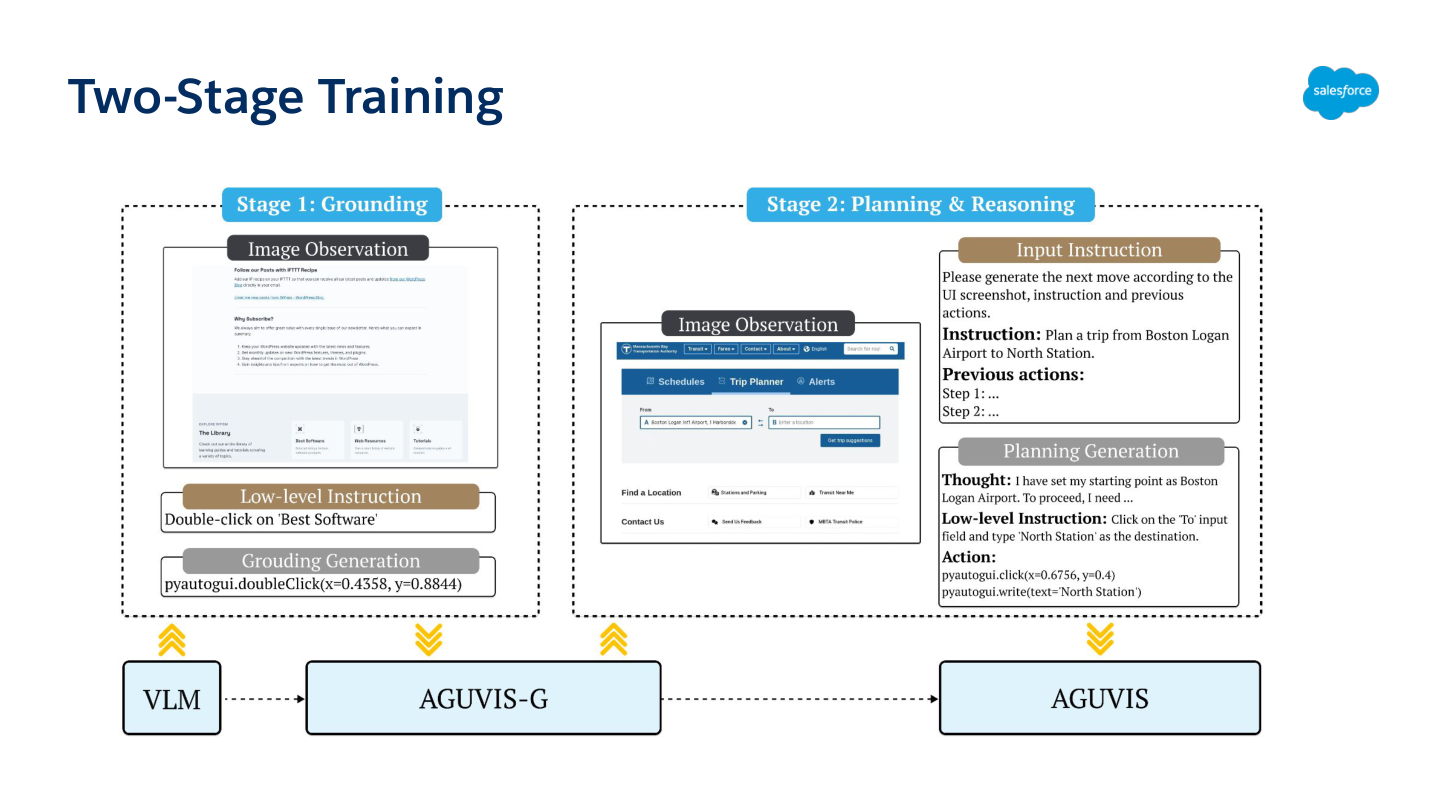
\includegraphics[width=0.78\textwidth]{figures/lec07_fig_008.png}
\caption{AGUVIS 先学 GUI grounding，再学 planning / reasoning，这是一种明确的 curriculum design。}
\end{figure}

AGUVIS 的第二个关键设计是 two-stage training。原因是 GUI grounding 与 high-level planning 的优化目标不同：前者更像视觉定位与 element grounding，后者更像多步 decision making。如果一开始就混在一起训，模型很容易只学到局部 pattern，而学不到稳定的 reasoning policy。

slides 还特别强调了 \textbf{inner monologue}：
\begin{figure}[H]
\centering
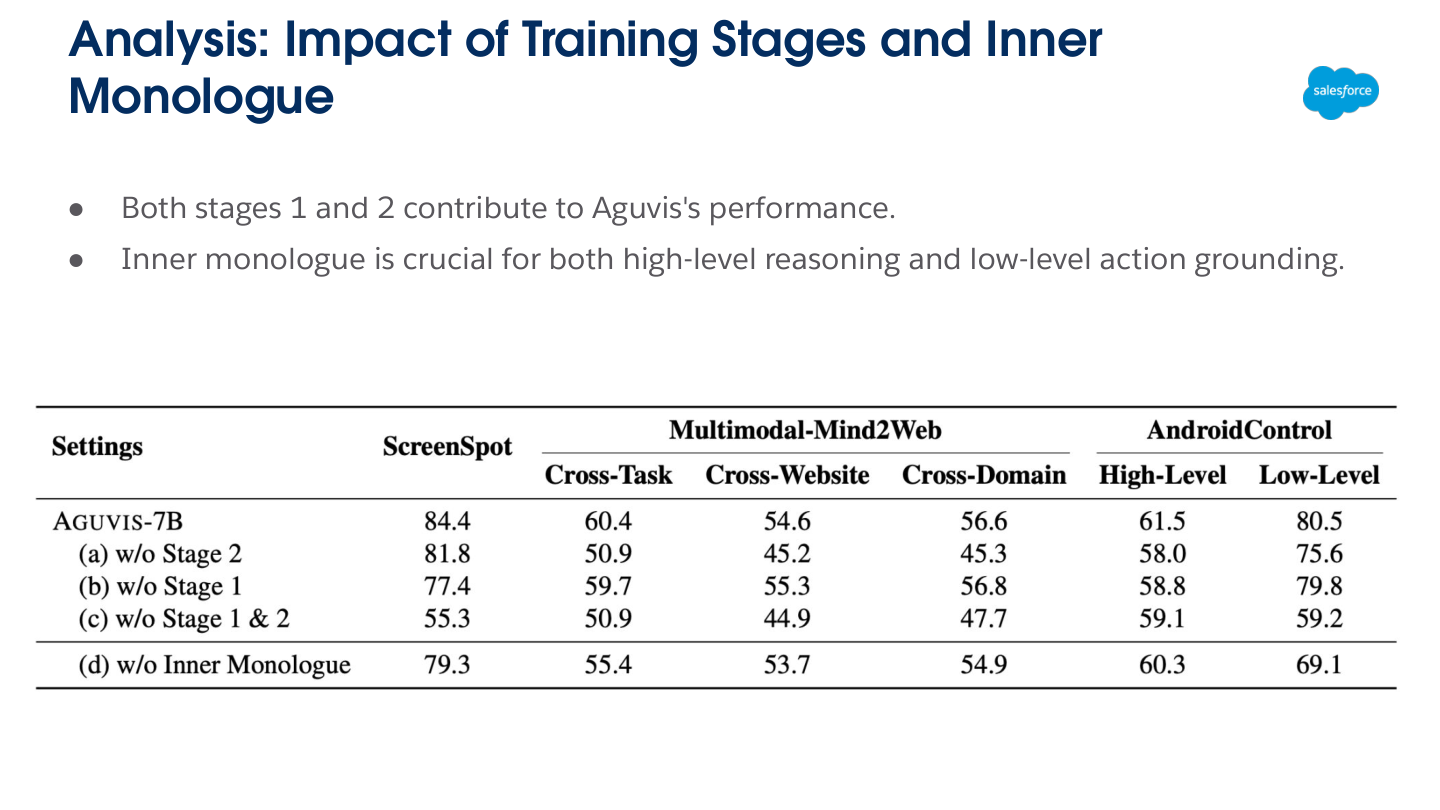
\includegraphics[width=0.78\textwidth]{figures/lec07_fig_009.png}
\caption{Inner monologue 不只是“多说两句”，而是连接高层 reasoning 与低层 grounding 的中间结构。}
\end{figure}

这点和很多读者的直觉相反。inner monologue 的作用不只是提升高层 reasoning，它还会改善低层 grounding。原因是：当模型显式写出自己正在寻找什么元素、当前屏幕上哪些区域相关、下一步想验证什么时，后续的坐标或元素选择就更少是盲点操作。

\begin{warningbox}{一个常见误解}
Pure-vision GUI agent 并不意味着“永远不需要文本”。它真正反对的是把不同平台的 HTML/AXTree/XML 当作不可替代的主表示，从而让 observation space 和 action space 在跨平台时失去统一性。
\end{warningbox}

\section{长视频与多模态 agent memory}

\subsection{xGen-MM-Vid：为什么长视频首先是 memory 问题}

讲者最后一部分表面上在讲 Video LLM，实则是在讨论 agent 的 \textbf{长程视觉记忆}。长视频任务和长程 agent 任务有一个共同困难：原始观测序列太长，不能原样喂给模型。于是 xGen-MM-Vid / BLIP-3-Video 的核心设计是通过 temporal encoder 把视频帧序列压缩成少量 token：
\[
z_{1:K}=f_\theta(v_{1:T}),\qquad K \ll T.
\]
这里 $v_{1:T}$ 是原始帧序列，$z_{1:K}$ 是压缩后的 temporal tokens。直觉上，这相当于给长视频设计一个更高层的 memory representation。

\begin{figure}[H]
\centering
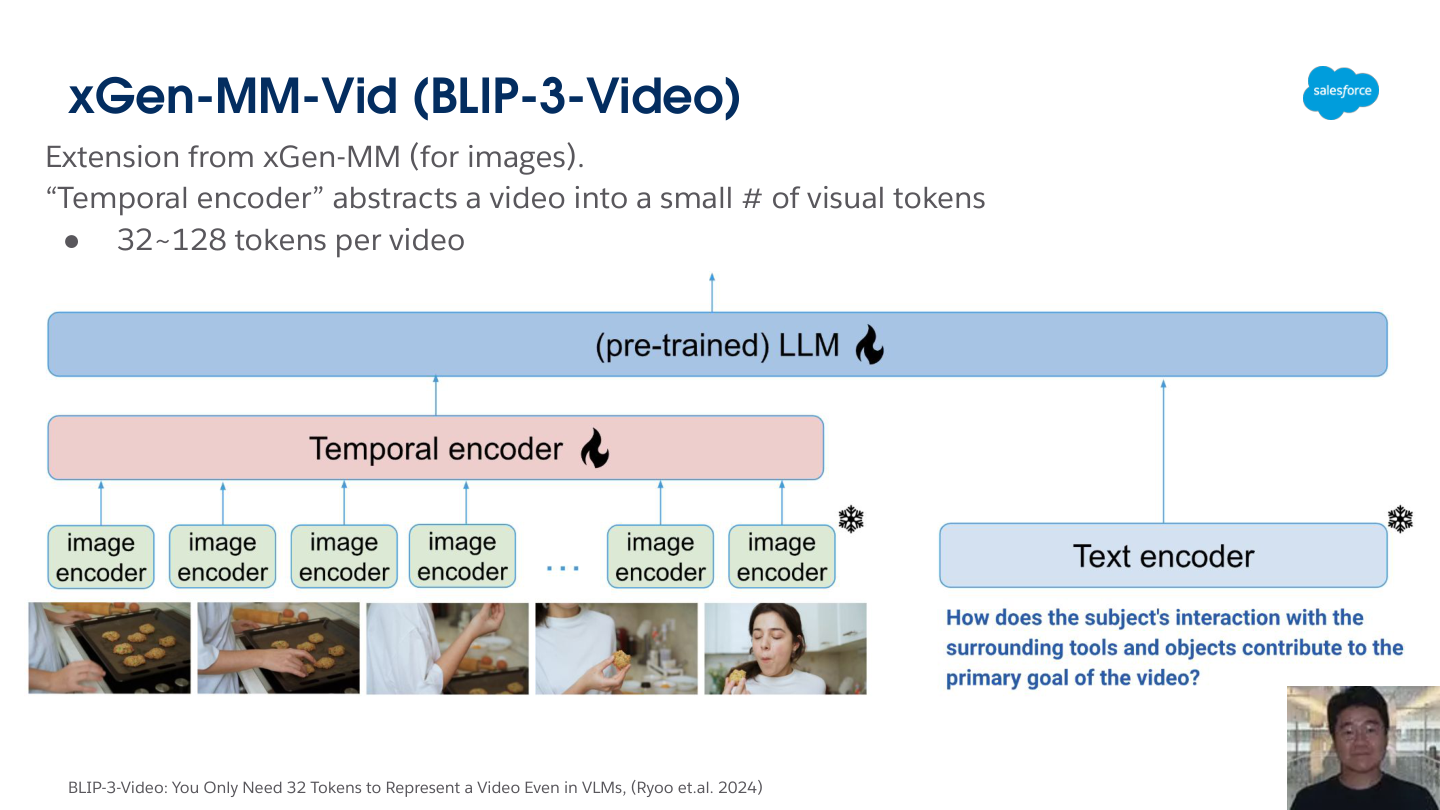
\includegraphics[width=0.78\textwidth]{figures/lec07_fig_010.png}
\caption{xGen-MM-Vid 通过 temporal encoder 把长视频压缩成很少的视觉 token，从而把 memory 问题变成可计算问题。}
\end{figure}

这与 GUI / OS agents 的联系在于：\textbf{agent 不能无限保留所有原始 observation，它必须学会压缩、筛选和重访。} 对 web tasks，压缩的是 history；对 long video，压缩的是 frame sequence；两者都在处理有限 context budget 下的 memory allocation。

\subsection{GenS：把 frame selection 变成条件生成}

如果 xGen-MM-Vid 关注长视频 token compression，\textbf{GenS} 则更像是在解决 \emph{instruction-conditioned frame selection}。slides 明确批评纯 CLIP-based sampling：它难以捕捉 temporal relation，也难以处理 multi-hop language reasoning。GenS 的做法是直接生成相关 frame spans 与其分数：
\[
\hat{\mathcal{I}}=\{(i, r_i)\}_{i=1}^{T},\qquad r_i\in[0,1].
\]
其中 $i$ 是帧索引或时间片，$r_i$ 是与用户指令相关的置信分数。这种写法意味着 frame selection 不再只是 embedding similarity，而是 \textbf{带语言条件的生成式 grounding}。

\begin{figure}[H]
\centering
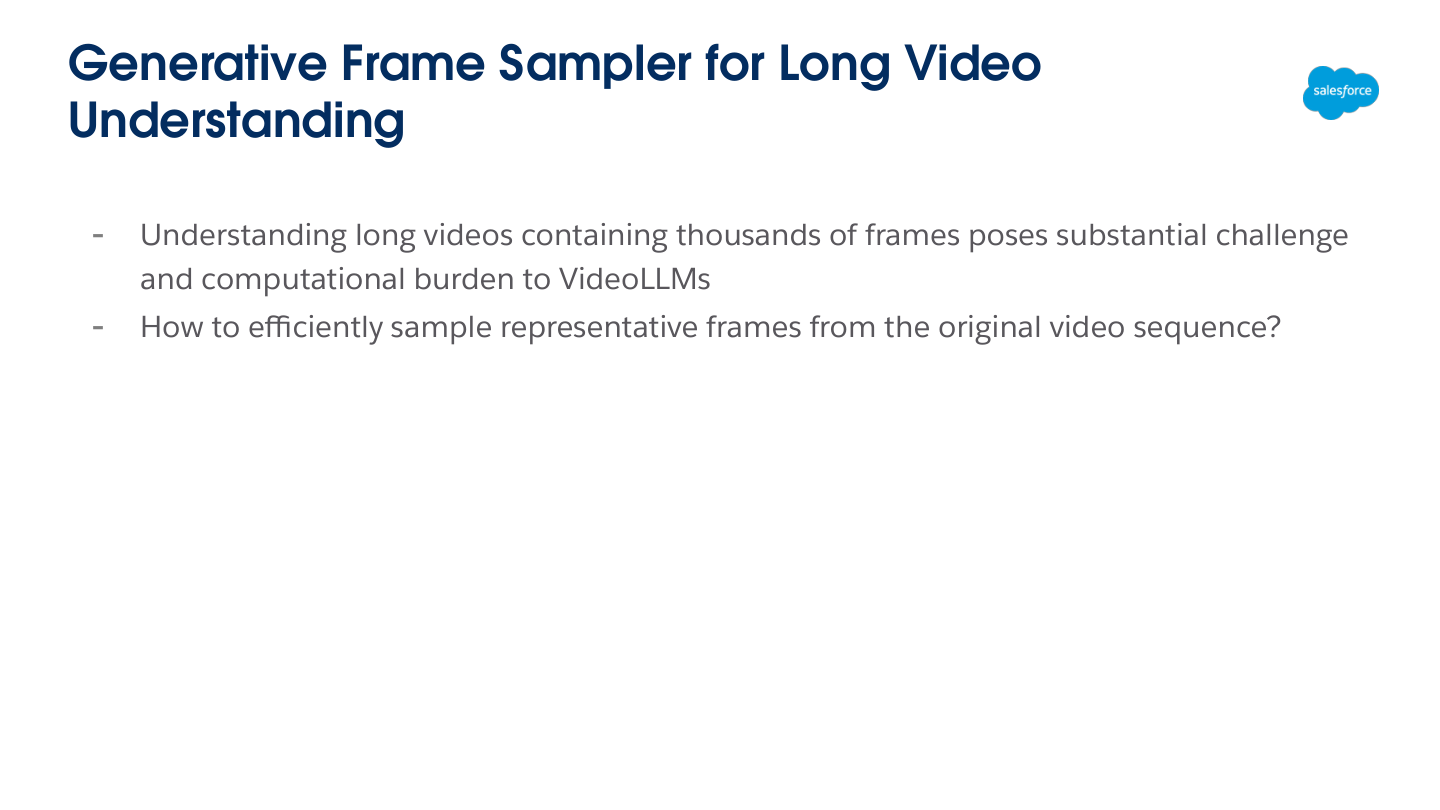
\includegraphics[width=0.78\textwidth]{figures/lec07_fig_011.png}
\caption{GenS 通过生成式方式预测 relevant frame spans，而不是只做相似度检索。}
\end{figure}

教材化地看，GenS 的重要性在于：它把 long-video grounding 明确纳入了 agent 设计问题。因为很多未来的 multimodal agents 不只看单张截图，而是需要在长视频、桌面录屏或复杂交互历史中定位与目标相关的时序片段。

\section{与核心 readings 的关系}

\subsection{OSWorld：为什么本讲把 benchmark 当作环境设计问题}

《OSWorld》是本讲前半段最核心的 reading。它的重要性不只是提供一个 leaderboard，而是重新定义了 multimodal computer-use agent 到底应该面对什么 environment。论文把 task setup、execution-based evaluation、跨应用 workflow 和真实操作系统状态放到中心位置，这恰好解释了为什么讲者要反复区分 web benchmark、OS benchmark 和 GUI grounding benchmark。

从教材角度看，OSWorld 给出的最大信息不是最强 baseline 只有多少分，而是 human-agent gap 的结构来源：\textbf{不是单纯语言理解不足，而是 grounding、操作知识和多步环境反馈处理能力同时落后。} 这也解释了为什么本讲不会把“会看图”与“会用电脑”混为一谈。

\subsection{AGUVIS：为什么 pure vision 不是“去掉文本”，而是统一 observation space}

《AGUVIS》则为本讲后半段的 GUI section 提供了最直接的 reading 支撑。它的核心立场不是“文本没用”，而是：如果 agent 长期依赖 HTML、AXTree、XML 这类平台特有表示，它就很难形成真正统一的跨平台学习问题。lecture 里关于 unified action space、inner monologue 和 two-stage training 的讨论，基本都能在这篇 paper 的 framing 中找到来源。

这篇 reading 还帮助我们更清楚地区分两类能力：一类是 \textbf{GUI grounding}，即能不能在视觉空间里定位正确目标；另一类是 \textbf{interactive reasoning}，即知道下一步为什么要点、点完之后如何继续。AGUVIS 的两阶段设计正是因为这两类能力虽然相关，但优化目标并不完全相同。

\subsection{两篇 readings 合在一起看，才能得到完整结论}

如果只看 OSWorld，你会更清楚 benchmark 和 environment realism 的问题；如果只看 AGUVIS，你会更清楚 observation 与 action representation 的问题。把两者合起来，lecture 想表达的完整结论才成立：\textbf{multimodal agent 的难点既不是纯 benchmark 设计，也不是纯模型架构设计，而是 environment、grounding、action space、training data 和 memory compression 的联立问题。}

\section{本章小结与跨讲联系}

本讲把 multimodal agents 的问题分成六个维度：environment、data、models、reasoning、grounding、memory。这个分法非常有启发性，因为它防止我们把一切都归结为“换个更强模型”。

与上一讲相比，这一讲进一步把问题从 \textbf{web agents} 推向 \textbf{computer-use agents} 与 \textbf{GUI agents}。上一讲强调 benchmark realism、inference-time search 和 synthetic tasks；这一讲则补上了 execution-based OS benchmarks、pure-vision grounding、action-call training 与 long-video memory。两讲放在一起，才构成一套较完整的 multimodal agent textbook view。

\section{复习题}
\begin{enumerate}
\item 为什么 OSWorld 比只有 demonstrations 的数据集更适合评估 computer-use agents？
\item execution-based evaluation 与字符串匹配相比，最大的优势是什么？
\item AgentTrek 的 guided replay 在数据生成中解决了什么问题？
\item CoTA 与普通 CoT 的关键差别是什么？
\item AGUVIS 为什么强调 pure-vision observation 和 unified action space？
\item xGen-MM-Vid 与 GenS 分别想解决长视频中的什么瓶颈？
\end{enumerate}

\section{深入思考题}
\begin{enumerate}
\item 如果一个模型在 OSWorld 上分数低，但在 GUI grounding benchmark 上分数高，你会如何诊断它的问题？
\item inner monologue 在 deployment-time 是否一定值得保留？在什么场景下它的成本可能超过收益？
\item 长视频 frame selection 与 web-agent search 能否被统一看作对有限预算的 inference-time allocation？
\end{enumerate}

\section{延伸阅读}
\begin{itemize}
\item OSWorld: Benchmarking Multimodal Agents for Open-Ended Tasks in Real Computer Environments.
\item AGUVIS: Unified Pure Vision Agents for Autonomous GUI Interaction.
\item AgentTrek: agent trajectory synthesis via guiding replay with web tutorials.
\item TACO / Synthetic Chains-of-Thought-and-Action.
\item BLIP-3-Video / xGen-MM-Vid.
\item Generative Frame Sampler for Long Video Understanding.
\end{itemize}
\end{document}
